%        File: main.tex
%     Created: mar abr 30 11:00  2013 C
% Last Change: mar abr 30 11:00  2013 C
%
\documentclass[12pt,a4paper]{article}

\usepackage[spanish]{babel}
\usepackage[utf8]{inputenc}
\usepackage{graphicx}
\usepackage{xcolor, colortbl}
\definecolor{azulito}{rgb}{0.8,0.8,0.8}
\usepackage{longtable}
\usepackage{amsfonts}
\usepackage{amssymb}
\usepackage{caption}
\usepackage{multicol}
\usepackage{fancyhdr}
\usepackage{multirow}
\usepackage[total={18cm,24cm},top=3cm,left=2cm]{geometry}
\setlength{\parskip}{\baselineskip}

\date{13 de mayo de 2013}
\title{Actividad 7.1\\
    Caída de conos\\
}
\author{Universidad Nacional Autónoma de México \\
    Facultad de Ciencias \\
    Amaro Alcalá David \\
    Equipo 4 \\
    Prof. Alejandro González y Hernández\\
    Ay. Ismael Ponce Rosas\\
    Laboratorio 2\\
    }

\newenvironment{Figure}
{\par\medskip\noindent\minipage{\linewidth}}
{\endminipage\par\medskip}

\newenvironment{Tabla}
{\par\medskip\noindent\minipage{\linewidth}}{\endminipage\par\medskip}
\pagestyle{fancy}

\fancyhead[CL]{David Amaro Alcal\'{a}}
\fancyhead[CR]{\textit{Actividad 7.1}}
\fancyhead[C]{Caída de conos de papel}

\begin{document}
        \begin{titlepage}
    \maketitle
\end{titlepage}

    \begin{multicols}{2}
        \begin{center}
    {\huge Caída de conos}\\
    {\normalsize David Amaro Alcalá}\\
    {\normalsize Laboratorio 2}\\
    dav1494@ciencias.unam.mx\\
\end{center}

\section*{Resumen}

Se dejarón caer tres conos con distinta masa pero la misma área
de contacto con el aire y se obtuvo su posición y el tiempo
con Tracker.

Se comprobo que la fuerza de resistencia del aire es directamente
proporcional al cuadrado y se obtuvo la constante de proporcionalidad.

Los valores obtenidos para la \textbf{velocidad terminal} son:

\begin{Tabla}
    \centering
    \begin{tabular}{|c|c|}
        \hline
        \rowcolor{azulito} Cono & Velocidad Terminal (m/s)  \\
        \hline 1 & -1.27384 \\
        \hline 2 & -1.42074 \\
        \hline 3 & -1.60727 \\
        \hline
    \end{tabular}
\end{Tabla}

Y también se obtuvieron los siguientes valores

\begin{Tabla}
    \centering
    \begin{tabular}{|c|c|}
        \hline 
        \rowcolor{azulito} Parámetro & Valor \\
        \hline $C_D$ & 0.776 \\
        \hline $r$ & 0.0095 \\
        \hline
    \end{tabular}
\end{Tabla}
 % Resumen
        \section{Introducción}

Aunque en la mayoría de casos estudiados se desprecia
la fuerza de resistencia del aire, pero a grandes velocidades
su intervención en el movimiento de un objeto es importante tomarla 
en cuenta.

La ecuación en caída libre de un objeto con resistencia es:

\begin{equation}
    F = W + f = -mg + rv^2
    \label{int_caidalibre}
\end{equation}

donde $m$ es la masa del objeto cayendo, $g$ la aceleración de la
gravedad, $r$ el coeficiente de fricción del fluido sobre el que se esta
cayendo y $v$ la velocidad del objeto.

En caída libre el objeto cayendo alcanza la llamada \textit{velocidad terminal}
debido a la fuerza de resistencia del aire.

Como es fácil ver, el cono alcanza esta velocidad $v_t$ cuando $a$ es cero, es decir
\[
    -mg + rv^2 = 0,
\]
desarrollando:
\[
    mg = rv^2_t
\]

$r$ se puede calcular con la siguiente expresión:

\begin{equation}
    r = \frac{\rho A C_D}{2}
    \label{int_calcoef}
\end{equation}

donde $\rho$ es la densidad del aire, $A$ es el área que tiene
contacto con el fluido y $C_D$ es un coeficiente de arrastre
que depende de la forma del objeto cayendo.

Despejando a $C_D$ obtenemos

\begin{equation}
    C_D = \frac{2r}{\rho A}
    \label{int_valorDeR}
\end{equation}

Que nos permitirá conocer este último coeficiente después de determinar
$r$.

Finalmente para concer el área de la superficie de contacto 
de los conos desarrollamos lo siguiente.

\begin{equation}
    A_c = \pi R g
    \label{AreaCono}
\end{equation}

donde $A_c$ es el área del cono, $R$ el radio del círculo.

También sabemos que:

\begin{equation}
    P = 2 \pi r
    \label{Perimetro}
\end{equation}

donde $P$ es el perímetro del cono y $r$
es el radio del círculo que formará al cono.

Otra expresión util es:

\begin{equation}
    S = r \theta
    \label{Arco}
\end{equation}

con $S$ el arco del círculo y $\theta$ el ángulo
de la parte que se mutilo al círculo base.
 % Introducción
        \section{Objetivo}

\begin{enumerate}
    \item Conocer la velocidad terminal de cada cono.
    \item Conocer el coeficiente $r$ de resistencia del aire y
    \item Conocer el valor $C_D$ del área de los conos.
\end{enumerate}
 % Objetivo
        \section{Exploración}

Con mayor área de contacto el cono disminui la velocidad en
menor tiempo.

Si el cono tenía un área de contacto grande, era necesario
incluir un poco de plastilina para que cayera sin que
se modificara su desplazamiento vertical.
 % Exploración
        \section{Descripción}

\subsection{Material}

\begin{enumerate}
    \item Compás.
    \item Tijeras.
    \item Dos hojas de papel.
    \item Cámara digital y tripie.
    \item Metro.
    \item Plastilina.
    \item Balanza.
\end{enumerate}

\subsection{Montaje experimental}

\begin{description}
    \item[Paso 1] Se fabricaron los conos de tal forma que todos
        tuvieran un radio $a$ constante, lo demás era necesario variarlo.
    \item[Paso 2] Se midieron las masa de los dos conos utilizados.
    \item[Paso 3] Se coloco la cámara y una regla paralela al lente de
        la cámara.
    \item[Paso 4] Dejar caer el cono desde el reposo a una altura $h$ constante.
    \item[Paso 5] Análisis de los videos con Tracker.
\end{description}
 % Descripción del experimento
        \section{Hipótesis}

\begin{enumerate}
    \item El valor de la fuerza es directamente proporcional al cuadrado
        de la velocidad.
    \item La fuerza es independiente de la masa del objeto que está
        cayendo y sólo depende del valor de su velocidad.
\end{enumerate}
 % Hipótesis
    \end{multicols}
        \section{Tablas}

\begin{table}
    \centering
    \begin{tabular}{|c|c|}
        \hline
        \rowcolor{azulito} Cono & Masa (kg) $\pm 5\times10^{-4}$ kg \\
        \hline Cono 1 & 0.00157 \\
        \hline Cono 2 & 0.00207 \\
        \hline Cono 3 & 0.00257 \\
        \hline
    \end{tabular}
    \caption{Masa de cada cono, medidas hechas con la
    báscula.}
    \label{tab:masa_cono}
\end{table}

\begin{longtable}{|c|c|c|c|}
        \hline
        \rowcolor{azulito} & Cono 1 & Cono 2 & Cono 3 \\
        \rowcolor{azulito} $t(s) \pm 0.0165$ s& $y(m) \pm 5\times10^{-4}$ m& $y(m) \pm  5\times10^{-4}$ m& $y(m) \pm 5\times10^{-4}$ m\\
        \endhead
        \hline 0 & 0 & 0 & 0 \\
        \hline 0.033 & -0.006 & -0.015 & -0.002 \\
        \hline 0.067 & -0.023 & -0.03 & -0.009 \\
        \hline 0.1 & -0.044 & -0.059 & -0.029 \\
        \hline 0.133 & -0.068 & -0.078 & -0.058 \\
        \hline 0.167 & -0.093 & -0.109 & -0.093 \\
        \hline 0.2 & -0.121 & -0.143 & -0.127 \\
        \hline 0.233 & -0.15 & -0.182 & -0.166 \\
        \hline 0.267 & -0.182 & -0.216 & -0.208 \\
        \hline 0.3 & -0.212 & -0.26 & -0.254 \\
        \hline 0.333 & -0.245 & -0.3 & -0.302 \\
        \hline 0.367 & -0.28 & -0.344 & -0.343 \\
        \hline 0.4 & -0.319 & -0.389 & -0.39 \\
        \hline 0.433 & -0.361 & -0.432 & -0.443 \\
        \hline 0.467 & -0.403 & -0.478 & -0.501 \\
        \hline 0.5 & -0.447 & -0.526 & -0.56 \\
        \hline 0.533 & -0.493 & -0.571 & -0.62 \\
        \hline 0.567 & -0.532 & -0.615 & -0.679 \\
        \hline 0.6 & -0.571 & -0.659 & -0.738 \\
        \hline 0.633 & -0.61 & -0.703 & -0.801 \\
        \hline 0.667 & -0.648 & -0.748 & -0.856 \\
        \hline 0.7 & -0.687 & -0.797 & -0.912 \\
        \hline 0.733 & -0.728 & -0.846 & -0.968 \\
        \hline 0.767 & -0.77 & -0.895 & -1.024 \\
        \hline 0.8 & -0.815 & -0.944 & -1.082 \\
        \hline 0.833 & -0.861 & -1.003 & -1.141 \\
        \hline 0.867 & -0.905 & -1.063 & -1.2 \\
        \hline 0.9 & -0.949 & -1.116 & -1.258 \\
        \hline 0.933 & -0.989 & -1.166 & -1.316 \\
        \hline 0.967 & -1.029 & -1.215 & -1.368 \\
        \hline 1 & -1.068 & -1.302 & -1.425 \\
        \hline 1.033 & -1.122 & -1.318 & -1.481 \\
        \hline 1.067 & -1.171 & -1.367 & -1.539 \\
        \hline 1.1 & -1.22 & -1.416 & -1.594 \\
        \hline 1.133 & -1.269 & -1.466 & -1.651 \\
        \hline 1.167 & -1.318 & -1.519 & -1.706 \\
        \hline 1.2 & -1.357 & -1.569 & -1.762 \\
        \hline 1.233 & -1.397 & -1.618 & -1.816 \\
        \hline 1.267 & -1.451 & -1.667 & -1.872 \\
        \hline 1.3 & -1.5 & -1.716 & -1.928 \\
        \hline 1.333 & -1.539 & -1.765 & -1.982 \\
        \hline 1.367 & -1.583 & -1.815 & -2.036 \\
        \hline 1.4 & -1.63 & -1.864 & -2.09 \\
        \hline 1.433 & -1.678 & -1.913 & -2.143 \\
        \hline 1.467 & -1.728 & -1.962 & -2.194 \\
        \hline 1.5 & -1.78 & -2.007 & -2.255 \\
        \hline 1.533 & -1.834 & -2.056 & -2.258 \\
        \hline 1.567 & -1.883 & -2.105 & -1.622 \\
        \hline
    \caption{Tabla con la posición y el tiempo de cada cono.}
    \label{tab:postiemcono}
\end{longtable}

Por la ecuación (\ref{int_caidalibre}) sabemos que la velocidad terminal es la
pendiente de la gráfica obtenida con los datos anteriores, entonces
se hace un ajuste lineal para obtener la ecuación de la recta y
su pendiente será el valor de la velocidad terminal. Las gráficas
pertenecen a la siguiente sección.

A continuación se listan las características de cada cono:

\begin{table}[h]
    \centering
    \begin{tabular}{c|c|c|}
        \cline{2-3}
        \rowcolor{azulito} & Altura (m) & Ángulo (rad) \\
        \hline \multicolumn{1}{|c|}{Cono 1} & 5 $\times 10^{-2}$ & $\frac{17 \pi}{45}$ \\
        \hline \multicolumn{1}{|c|}{Cono 2} & 3 $\times 10^{-2}$ & $\frac{14 \pi}{45}$ \\
        \hline \multicolumn{1}{|c|}{Cono 3} & 7 $\times 10^{-2}$ & $\frac{7 \pi}{18}$ \\
        \hline
    \end{tabular}
    \caption{Tabla con las carácteristicas que contaba cada cono
    al ser lanzado.}
    \label{tab:ConoCar}
\end{table}
 % Tablas
        \section{Gráficas}

Se grafican los datos de \ref{tab:postiemcono} y la velocidad.

\clearpage
\begin{figure}[h!]
    \centering
    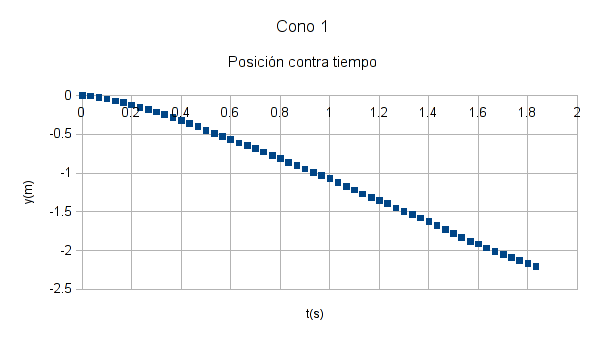
\includegraphics{pos_time1}
    \caption{Gráfica de posición contra tiempo para el cono 1. Se puede 
    observar que a partir de $t$ igual a 0.4 s se alcanza la velocidad
    terminal.}
    \label{fig:posl_cono1}
\end{figure}

\begin{figure}[h!]
    \centering
    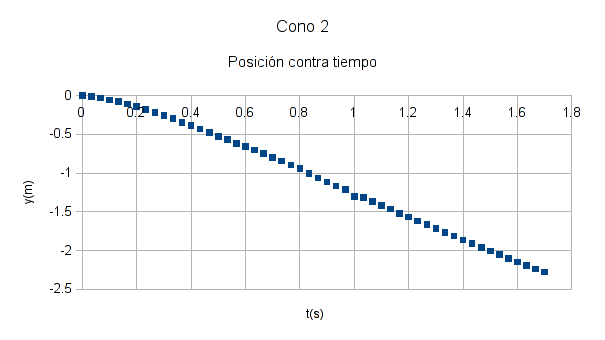
\includegraphics{pos_time2}
    \caption{De nuevo se observa que el cono alcanza su velocidad terminal en
    el instante $t$ igual a 0.3 s.}
    \label{fig:pos1_cono2}
\end{figure}

\begin{figure}[h!]
    \centering
    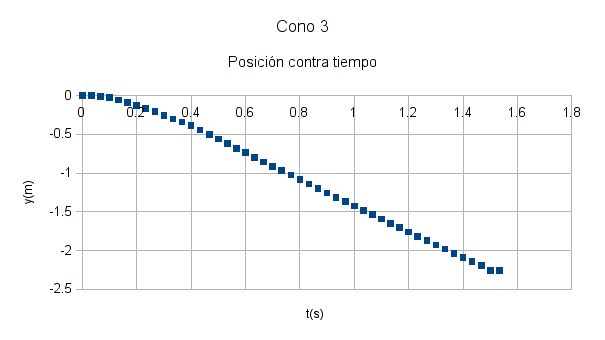
\includegraphics{pos_time3}
    \caption{Gráfica de posición contra tiempo del cono número 3.
    La velocidad terminal es alcanzada en el tiempo 0.25 s.}
    \label{fig:pos1_cono3}
\end{figure}
 % Gráficas
        \section{Interpretación de gráficas}

Como se puede observar en las gráficas de la sección anterior, 
al pasar un tiempo dado, los conos alcanzan su velocidad terminal.

Esto nos permite ajustar una recta a esos datos para conocer su velocidad
terminal.
 % Interpretación de las gráficas
        \section{Cálculo de parámetros}

\subsection{Velocidad}

Primero se tiene que conocer la velocidad en cada instante del movimiento.

Para eso se cálcula cada velocidad utilizando la expresión $v = \frac{\Delta x}{\Delta t}$

\clearpage
\begin{longtable}{|c|c|c|c|c|c|c|}
    \hline
    \rowcolor{azulito} & \multicolumn{2}{c|}{Cono 1} & \multicolumn{2}{c|}{Cono 2} & \multicolumn{2}{c|}{Cono 3} \\
    \hline
    \rowcolor{azulito} t(s) & v (m/s) & $\delta v$ & v (m/s) & $\delta v$ & v (m/s) & $\delta v$ \\
    \endhead
    \hline 0.00 & 0.000 & 0.0000 & 0.000 & 0.0000 & 0.000 & 0.0000 \\
    \hline 0.03 & -0.182 & 0.4997 & -0.455 & 0.4993 & -0.061 & 0.4999 \\
    \hline 0.07 & -0.515 & 0.2460 & -0.224 & 0.2459 & -0.104 & 0.2462 \\
    \hline 0.10 & -0.636 & 0.1648 & -0.290 & 0.1647 & -0.200 & 0.1649 \\
    \hline 0.13 & -0.727 & 0.1239 & -0.143 & 0.1238 & -0.218 & 0.1239 \\
    \hline 0.17 & -0.758 & 0.0986 & -0.186 & 0.0986 & -0.210 & 0.0986 \\
    \hline 0.20 & -0.848 & 0.0823 & -0.170 & 0.0823 & -0.170 & 0.0823 \\
    \hline 0.23 & -0.879 & 0.0707 & -0.167 & 0.0706 & -0.167 & 0.0707 \\
    \hline 0.27 & -0.970 & 0.0617 & -0.127 & 0.0616 & -0.157 & 0.0617 \\
    \hline 0.30 & -0.909 & 0.0549 & -0.147 & 0.0549 & -0.153 & 0.0549 \\
    \hline 0.33 & -1.000 & 0.0494 & -0.120 & 0.0494 & -0.144 & 0.0494 \\
    \hline 0.37 & -1.061 & 0.0449 & -0.120 & 0.0448 & -0.112 & 0.0448 \\
    \hline 0.40 & -1.182 & 0.0412 & -0.113 & 0.0411 & -0.118 & 0.0411 \\
    \hline 0.43 & -1.273 & 0.0380 & -0.099 & 0.0380 & -0.122 & 0.0380 \\
    \hline 0.47 & -1.273 & 0.0352 & -0.099 & 0.0352 & -0.124 & 0.0352 \\
    \hline 0.50 & -1.333 & 0.0329 & -0.096 & 0.0329 & -0.118 & 0.0329 \\
    \hline 0.53 & -1.394 & 0.0309 & -0.084 & 0.0309 & -0.113 & 0.0308 \\
    \hline 0.57 & -1.182 & 0.0290 & -0.078 & 0.0290 & -0.104 & 0.0290 \\
    \hline 0.60 & -1.182 & 0.0274 & -0.073 & 0.0274 & -0.098 & 0.0274 \\
    \hline 0.63 & -1.182 & 0.0260 & -0.070 & 0.0260 & -0.100 & 0.0260 \\
    \hline 0.67 & -1.152 & 0.0247 & -0.067 & 0.0247 & -0.082 & 0.0246 \\
    \hline 0.70 & -1.182 & 0.0235 & -0.070 & 0.0235 & -0.080 & 0.0235 \\
    \hline 0.73 & -1.242 & 0.0224 & -0.067 & 0.0224 & -0.076 & 0.0224 \\
    \hline 0.77 & -1.273 & 0.0214 & -0.064 & 0.0214 & -0.073 & 0.0214 \\
    \hline 0.80 & -1.364 & 0.0206 & -0.061 & 0.0206 & -0.073 & 0.0205 \\
    \hline 0.83 & -1.394 & 0.0197 & -0.071 & 0.0197 & -0.071 & 0.0197 \\
    \hline 0.87 & -1.333 & 0.0190 & -0.069 & 0.0190 & -0.068 & 0.0190 \\
    \hline 0.90 & -1.333 & 0.0183 & -0.059 & 0.0183 & -0.064 & 0.0183 \\
    \hline 0.93 & -1.212 & 0.0176 & -0.054 & 0.0176 & -0.062 & 0.0176 \\
    \hline 0.97 & -1.212 & 0.0170 & -0.051 & 0.0170 & -0.054 & 0.0170 \\
    \hline 1.00 & -1.182 & 0.0164 & -0.087 & 0.0164 & -0.057 & 0.0164 \\
    \hline 1.03 & -1.636 & 0.0159 & -0.015 & 0.0159 & -0.054 & 0.0159 \\
    \hline 1.07 & -1.485 & 0.0154 & -0.046 & 0.0154 & -0.054 & 0.0154 \\
    \hline 1.10 & -1.485 & 0.0149 & -0.045 & 0.0149 & -0.050 & 0.0149 \\
    \hline 1.13 & -1.485 & 0.0145 & -0.044 & 0.0145 & -0.050 & 0.0145 \\
    \hline 1.17 & -1.485 & 0.0141 & -0.045 & 0.0141 & -0.047 & 0.0141 \\
    \hline 1.20 & -1.182 & 0.0137 & -0.042 & 0.0137 & -0.047 & 0.0137 \\
    \hline 1.23 & -1.212 & 0.0133 & -0.040 & 0.0133 & -0.044 & 0.0133 \\
    \hline 1.27 & -1.636 & 0.0130 & -0.039 & 0.0130 & -0.044 & 0.0130 \\
    \hline 1.30 & -1.485 & 0.0126 & -0.038 & 0.0126 & -0.043 & 0.0126 \\
    \hline 1.33 & -1.182 & 0.0123 & -0.037 & 0.0123 & -0.041 & 0.0123 \\
    \hline 1.37 & -1.333 & 0.0120 & -0.037 & 0.0120 & -0.040 & 0.0120 \\
    \hline 1.40 & -1.424 & 0.0117 & -0.035 & 0.0117 & -0.039 & 0.0117 \\
    \hline 1.43 & -1.455 & 0.0115 & -0.034 & 0.0115 & -0.037 & 0.0115 \\
    \hline 1.47 & -1.515 & 0.0112 & -0.033 & 0.0112 & -0.035 & 0.0112 \\
    \hline 1.50 & -1.576 & 0.0110 & -0.030 & 0.0110 & -0.041 & 0.0109 \\
    \hline 1.53 & -1.636 & 0.0107 & -0.032 & 0.0107 & -0.002 & 0.0107 \\
    \hline 1.57 & -1.485 & 0.0105 & -0.031 & 0.0105 & 0.0105 & \\
    \hline 1.60 & -1.061 & 0.0103 & -0.028 & & & \\
    \hline 1.63 & -1.485 & 0.0101 & -0.027 & & & \\
    \hline 1.67 & -1.364 & 0.0099 & -0.027 & & & \\
    \hline 1.70 & -1.182 & 0.0097 & -0.023 & & & \\
    \hline 1.73 & -1.182 & 0.0095 &        &        &        & \\
    \hline 1.77 & -1.212 & 0.0093 &        &        &        & \\
    \hline 1.80 & -1.182 & 0.0091 &        &        &        & \\
    \hline 1.83 & -1.273 & 0.0090 &        &        &        & \\
    \hline
    \caption{Velocidades de cada cono calculadas a partir
    de su posición.}
    \label{tab:Vel_Pos}
\end{longtable}
\subsection{Fuerza}

Para poder conocer la fuerza de resistencia que presenta el
aire al cono, obtenemos los valores de la velocidad en cada instante
de tiempo dado.

\begin{figure}[h!]
    \centering
    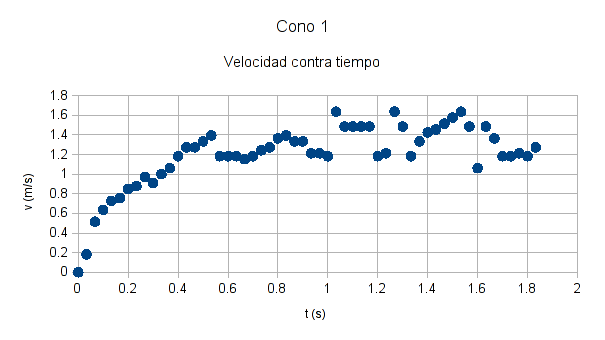
\includegraphics{vel_cono1}
    \caption{La grafica de la velocidad contra tiempo muestra que la velocidad terminal
    fue alcanzada a partir del tiempo 0.567 s y que los valores a partir de este
    tiempo se encuentran en nuestro rango de incertidumbre. Esto nos indica que el
    cono alcanzo su velocidad terminal en ese tiempo.}
    \label{fig:VelCono1}
\end{figure}

\begin{figure}[h!]
    \centering
    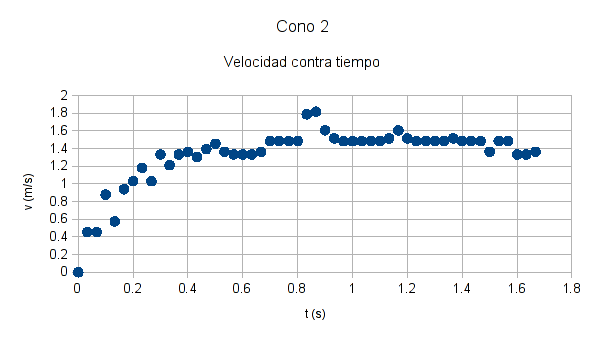
\includegraphics{vel_cono2}j
    \caption{Se observa que llegado el tiempo 0.667 s los valores de velocidad se encuentran
    dentro del rango de incertidumbre, esto nos permite concluir que 
    el cono alcanza su velocidad terminal.}
    \label{fig:VelCono2}
\end{figure}

\begin{figure}[h!]
    \centering
    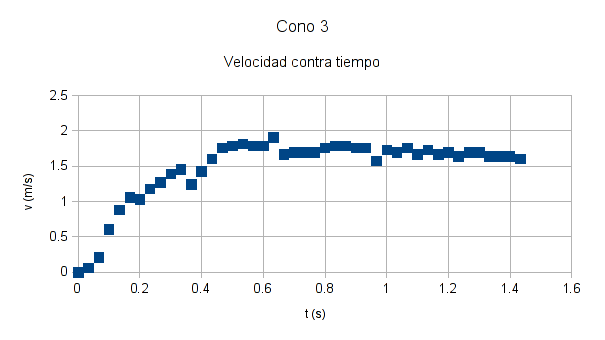
\includegraphics{vel_cono3}
    \caption{Grafica de la velocidad contra tiempo del cono 3 en la que observamos que 
    pasado un tiempo 0.700 s su velocidad se encuentra en un rango que se encuentra contenido
    dentro de las incertidumbres calculadas mostrando que alcanzo su velocidad terminal.}
    \label{fig:VelCono3}
\end{figure}
\subsection{Valor de $r$}

Ajustamos un recta a los valores graficados en
\ref{fig:posl_cono1}, \ref{fig:pos1_cono2} y \ref{fig:pos1_cono3}.
con la pendiente de dichas rectas obtenemos la velocidad
terminal de cada cono, así sustituyendo en las ecuaciones
\ref{int_valorDeR}.

\begin{table}
    \centering
    \begin{tabular}{|c|c|}
        \hline
        \rowcolor{azulito} Cono & Velocidad Terminal (m/s) \\
%         \hline 1 & -1.27384 \\
%         \hline 2 & -1.42074 \\
%         \hline 3 & -1.60727 \\
        \hline 1 & -1.273 \\
        \hline 2 & -1.420 \\
        \hline 3 & -1.607 \\
        \hline
    \end{tabular}
    \caption{En esta tabla se muestran los valores
    de la pendiente de la recta ajustada a los datos
    obtenidos en las tablas \ref{tab:postiemcono}.}
    \label{tab:VelTerminal}
\end{table}

Una vez conocidos las velocidades terminales de cada uno de los
conos, vamos a buscar conocer un valor de $r$ que nos permita
igualar la fuerza de atracción gravitacional con una fuerza que 
sea proporcional al cuadrado de la velocidad.

Se propone un valor para $r$ de 0.0095 y se multiplica este
valor por $v^2$ y se compara con la fuerza gravitacional que
sufre el cono.
\subsection{Valor de $C_D$}

Ya con el valor de $r$ bien definido, podemos conocer el
$C_D$, con la expresión \ref{int_valorDeR}:

Pero antes debemos calcular el área de los conos, para eso
hacemos uso de las expresiones \ref{AreaCono}, \ref{Perimetro}
y \ref{Arco}.

$\frac{31 \pi}{18}(0.1 m) = 2\pi R$
entonces $R = \frac{31}{360} \approx 0.086 m$

Y ahora si podemos obtener el área:

$A = \pi (0.086 m) (0.1 m) = \pi \frac{31}{3600} \approx 0.027m^2$

Entonces nuestro valor de $C_D$ es:

$ = \frac{2r}{\rho A} = \frac{2(0.0105\frac{kg}{m}}{1\frac{kg}{m^3}(0.027 m^2}) \approx 0.776$
 % Cálculo de parámetros
        \section{Resultados}

Se obtuvieron los valores de la velocidad
terminal para cada cono y también el valor de $r$.
 % Resultados
        \section{Análisis de los resultados}

Se obtuvo que esta fuerza es independiente de la masa, lo único
que afecta a esta fuerza es la velocidad que tiene el cono.
 % Análisis de los resultados
        \section{Conclusiones}

\begin{enumerate}
    \item Se encontró que la fuerza de resistencia del aire es
        independiente de la masa del objeto que está cayendo.
    \item La fuerza es directamente proporcional al cuadrado de 
        la velocidad que lleva el objeto al caer.
\end{enumerate}
 % Conclusiones
        \begin{thebibliography}{X}
        \bibitem[Ba]{Baird} \textsc{D. C. Baird} 
        \textit{Experimentación. Una introducción a la teoría
        de mediciones y al diseño de experimentos.}
        \bibitem[Re]{Resnick} \textsc{Resnick, R., Halliday, D,
        Krane, S.}
        \textit{Física \textbf{1}}
\end{thebibliography}
 % Bibliografía / Referencias
\end{document}
